\documentclass[11pt,reqno]{amsart}
\usepackage{amsfonts,amsmath,amssymb,amsbsy,amstext,amsthm,mathtools}
\usepackage{accents,color,enumerate,enumitem,float,fullpage,verbatim}

\usepackage{url}
\usepackage[colorlinks=true,hyperindex, linkcolor=magenta, pagebackref=false, citecolor=cyan]{hyperref}
\usepackage[alphabetic,lite]{amsrefs} 

%\usepackage{eucal,bm,kpfonts,mathbbol}

\usepackage{tikz,tikz-cd}	
\usetikzlibrary{positioning, matrix, shapes}         								    				
\usetikzlibrary{arrows,calc,matrix}

\usepackage{lscape}

\usepackage{microtype}


\usepackage{titlesec}		
\setcounter{secnumdepth}{4}						     					% Allows one to use nice section titles
\titleformat{\section}[block]{\scshape\bfseries\filcenter}{\thesection.}{1em}{}		% Creates section titles
\titleformat{\subsection}[runin]{\scshape\bfseries}{\thesubsection}{1em}{}			% Creates subsection titles
\titleformat{\subsubsection}[runin]{\scshape\bfseries}{\thesubsubsection}{1em}{}			% Creates subsection titles

\usepackage[titles]{tocloft}								     					% Creates table of fancy contents
\setcounter{tocdepth}{4}
\renewcommand{\contentsname}{}	     					% Renames and centers title of ToC

\usepackage{multirow}
\usepackage{array}
\usepackage{booktabs}
\newcolumntype{M}[1]{>{\centering\arraybackslash}m{#1}}
\newcolumntype{N}{@{}m{0pt}@{}}
\usepackage{diagbox}
\usepackage{cancel}

\newtheorem{lemma}{Lemma}[section]
\newtheorem{theorem}[lemma]{Theorem}
\newtheorem{goalTheorem}[lemma]{Goal Theorem}
\newtheorem{prop}[lemma]{Proposition}
\newtheorem{cor}[lemma]{Corollary}
\newtheorem{conj}[lemma]{Conjecture}
\newtheorem{claim}[lemma]{Claim}
\newtheorem{defn}[lemma]{Definition} 
\newtheorem{notation}[lemma]{Notation} 
\newtheorem{exercise}[lemma]{Exercise}
\newtheorem{question}[lemma]{Question}
\newtheorem*{assumption}{Assumption}
\newtheorem{principle}[lemma]{Principle}
\newtheorem{heuristic}[lemma]{Heuristic}

\newtheorem{theoremalpha}{Theorem}
\newtheorem{corollaryalpha}[theoremalpha]{Corollary}
\renewcommand{\thetheoremalpha}{\Alph{theoremalpha}}

\theoremstyle{remark}
\newtheorem{remark}[lemma]{Remark}
\newtheorem{example}[lemma]{Example}
\newtheorem{cexample}[lemma]{Counterexample}

% Commands
\newcommand{\initial}{\operatorname{in}}
\newcommand{\NF}{\operatorname{NF}}
\newcommand{\HF}{\operatorname{HF}}
\newcommand{\Hilb}{\operatorname{Hilb}}
\newcommand{\depth}{\operatorname{depth}}
\newcommand{\reg}{\operatorname{reg}}
\newcommand{\Span}{\operatorname{span}}
\newcommand{\img}{\operatorname{img}}
\newcommand{\inn}{\operatorname{in}}

\newcommand{\length}{\operatorname{length}}
\newcommand{\coker}{\operatorname{coker}}
\newcommand{\adeg}{\operatorname{adeg}}
\newcommand{\pdim}{\operatorname{pdim}}
\newcommand{\Spec}{\operatorname{Spec}}
\newcommand{\Ext}{\operatorname{Ext}}
\newcommand{\Tor}{\operatorname{Tor}}
\newcommand{\LT}{\operatorname{LT}}
\newcommand{\im}{\operatorname{im}}
\newcommand{\NS}{\operatorname{NS}}
\newcommand{\Frac}{\operatorname{Frac}}
\newcommand{\Khar}{\operatorname{char}}
\newcommand{\Proj}{\operatorname{Proj}}
\newcommand{\id}{\operatorname{id}}
\newcommand{\Div}{\operatorname{Div}}
\newcommand{\Kl}{\operatorname{Cl}}
\newcommand{\tr}{\operatorname{tr}}
\newcommand{\Tr}{\operatorname{Tr}}
\newcommand{\Supp}{\operatorname{Supp}}
\newcommand{\ann}{\operatorname{ann}}
\newcommand{\Gal}{\operatorname{Gal}}
\newcommand{\Pic}{\operatorname{Pic}}
\newcommand{\QQbar}{{\overline{\mathbb Q}}}
\newcommand{\Br}{\operatorname{Br}}
\newcommand{\Bl}{\operatorname{Bl}}
\newcommand{\Kox}{\operatorname{Cox}}
\newcommand{\conv}{\operatorname{conv}}
\newcommand{\getsr}{\operatorname{Tor}}
\newcommand{\diam}{\operatorname{diam}}
\newcommand{\Hom}{\operatorname{Hom}} %done
\newcommand{\sheafHom}{\mathcal{H}om}
\newcommand{\Gr}{\operatorname{Gr}}
\newcommand{\rank}{\operatorname{rank}} 
\newcommand{\codim}{\operatorname{codim}}
\newcommand{\Sym}{\operatorname{Sym}} %done
\newcommand{\GL}{{GL}}
\newcommand{\Prob}{\operatorname{Prob}}
\newcommand{\Density}{\operatorname{Density}}
\newcommand{\Syz}{\operatorname{Syz}}
\newcommand{\pd}{\operatorname{pd}}
\newcommand{\supp}{\operatorname{supp}}
\newcommand{\cone}{\operatorname{\textbf{cone}}}
\newcommand{\Res}{\operatorname{Res}}
\newcommand{\HS}{\operatorname{HS}}
\newcommand{\Cl}{\operatorname{Cl}}
\newcommand{\oO}{\operatorname{O}}

\newcommand{\defi}[1]{\textsf{#1}} % for defined terms

\newcommand{\remd}{\operatorname{remd}}
\newcommand{\colim}{\operatorname{colim}}
\newcommand{\trideg}{\operatorname{tri.deg}}
\newcommand{\indeg}{\operatorname{index.deg}}
\newcommand{\moddeg}{\operatorname{mod.deg}}
\newcommand{\Desc}{\operatorname{Desc}}
\newcommand{\inter}{\operatorname{int}}
\newcommand{\Nef}{\operatorname{Nef}}
\newcommand{\Jac}{\operatorname{Jac}}
\newcommand{\Cox}{\operatorname{Cox}}

\newcommand{\doot}{\bullet}

\newcommand{\Alt}{\bigwedge\nolimits}
\newcommand{\Set}{\text{\bf Set}}										% Category of Sets
\newcommand{\Sch}{\text{\bf Sch}}										% Category of Abelian Groups
\newcommand{\Mod}[1]{\ (\mathrm{mod}\ #1)}




%%%%%%%%%%%%%%%%%%%%%%%%%%%%%% Letters  %%%%%%%%%%%%%%%%%%%%%%%%%%%%%%%%%%%%%%%%%%%%
%%%%%%%%%%%%%%%%%%%%%%%%%%%%%%%%%%%%%%%%%%%%%%%%%%%%%%%%%%%%%%%%%%%%%%%%%%%%%%
\newcommand{\ff}{\mathbf f}
\newcommand{\kk}{\mathbf k}
\renewcommand{\aa}{\mathbf a}
\newcommand{\bb}{\mathbf b}
\newcommand{\cc}{\mathbf c}
\newcommand{\dd}{\mathbf d}
\newcommand{\ee}{\mathbf e}
\newcommand{\vv}{\mathbf v}
\newcommand{\ww}{\mathbf w}
\newcommand{\xx}{\mathbf x}
\newcommand{\yy}{\mathbf y}
\newcommand{\rr}{\mathbf r}
\newcommand{\ii}{\mathbf i}
\newcommand{\nn}{\mathbf n}
\newcommand{\pp}{\mathbf p}
\newcommand{\mm}{\mathbf m}
\newcommand{\fF}{\mathbf F}
\newcommand{\gG}{\mathbf G}
\newcommand{\eE}{\mathbf E}
\newcommand{\qQ}{\mathbf Q}
\newcommand{\tT}{\mathbf T}
\renewcommand{\tt}{\mathbf t}
\newcommand{\one}{\mathbf 1}
\newcommand{\zero}{\mathbf 0}

\renewcommand{\H}{\operatorname{H}}
\newcommand{\OO}{\operatorname{O}}
\newcommand{\oo}{\operatorname{o}}


%%%% Caligraphic Fonts - i.e. ????. %%%%%
\newcommand{\cA}{\mathcal{A}}
\newcommand{\cB}{\mathcal{B}}
\newcommand{\cC}{\mathcal{C}}
\newcommand{\cD}{\mathcal{D}}
\newcommand{\cE}{\mathcal{E}}
\newcommand{\cF}{\mathcal{F}}
\newcommand{\cG}{\mathcal{G}}
\newcommand{\cH}{\mathcal{H}} 
\newcommand{\cI}{\mathcal{I}}
\newcommand{\cJ}{\mathcal{J}}
\newcommand{\cK}{\mathcal{K}}
\newcommand{\cL}{\mathcal{L}}
\newcommand{\cM}{\mathcal{M}}
\newcommand{\cN}{\mathcal{N}}
\renewcommand{\O}{\mathcal{O}}
\newcommand{\cP}{\mathcal{P}}
\newcommand{\cQ}{\mathcal{Q}}
\newcommand{\cR}{\mathcal{R}}
\newcommand{\cS}{\mathcal{S}}
\newcommand{\cT}{\mathcal{T}}
\newcommand{\U}{\mathcal{U}} 		% Notice this is different
\newcommand{\cV}{\mathcal{V}}
\newcommand{\cW}{\mathcal{W}}
\newcommand{\cX}{\mathcal{X}}
\newcommand{\cY}{\mathcal{Y}}
\newcommand{\cZ}{\mathcal{Z}}

%%%% Blackboard Fonts - i.e. Real Numbers, Integers, etc. %%%%%
\newcommand{\A}{\mathbb{A}}
\newcommand{\B}{\mathbb{B}}
\newcommand{\C}{\mathbb{C}}
\newcommand{\D}{\mathbb{D}}
\newcommand{\E}{\mathbb{E}}
\newcommand{\F}{\mathbb{F}}
\newcommand{\G}{\mathbb{G}}
\newcommand{\I}{\mathbb{I}}
\newcommand{\J}{\mathbb{J}}
\newcommand{\K}{\mathbb{K}}
\renewcommand{\L}{\mathbb{L}}
\newcommand{\M}{\mathbb{M}}
\newcommand{\N}{\mathbb{N}}
\newcommand{\bO}{\mathbb{O}}		% Notice this is \bO
\renewcommand{\P}{\mathbb{P}}
\newcommand{\Q}{\mathbb{Q}}
\newcommand{\R}{\mathbb{R}}
\newcommand{\T}{\mathbb{T}}
\newcommand{\bU}{\mathbb{U}}		% Notice this is \bU
\newcommand{\V}{\mathbb{V}}
\newcommand{\W}{\mathbb{W}}
\newcommand{\X}{\mathbb{X}}
\newcommand{\Y}{\mathbb{Y}}
\newcommand{\Z}{\mathbb{Z}}

 %%%% Sarif Fonts - i.e. ???? %%%%%
\newcommand{\sA}{\mathsf{A}}
\newcommand{\sB}{\mathsf{B}}
\newcommand{\sC}{\mathsf{C}}
\newcommand{\sD}{\mathsf{D}}
\newcommand{\sE}{\mathsf{E}}
\newcommand{\sF}{\mathsf{F}}
\newcommand{\sG}{\mathsf{G}}
\newcommand{\sH}{\mathsf{H}} 
\newcommand{\sI}{\mathsf{I}}
\newcommand{\sJ}{\mathsf{J}}
\newcommand{\sK}{\mathsf{K}}
\newcommand{\sL}{\mathsf{L}}
\newcommand{\sM}{\mathsf{M}}
\newcommand{\sN}{\mathsf{N}}
\newcommand{\sO}{\mathsf{O}}
\newcommand{\sP}{\mathsf{P}}
\newcommand{\sQ}{\mathsf{Q}}
\newcommand{\sR}{\mathsf{R}}
\newcommand{\sS}{\mathsf{S}}
\newcommand{\sT}{\mathsf{T}}
\newcommand{\sU}{\mathsf{U}} 
\newcommand{\sV}{\mathsf{V}}
\newcommand{\sW}{\mathsf{W}}
\newcommand{\sX}{\mathsf{X}}
\newcommand{\sY}{\mathsf{Y}}
\newcommand{\sZ}{\mathsf{Z}}
 
 %%%% Fraktur Fonts - i.e. maximal ideals, prime ideals, etc. %%%%%
\newcommand{\cl}{\mathfrak{cl}}
\newcommand{\g}{\mathfrak{g}}
\newcommand{\h}{\mathfrak{h}}
\newcommand{\m}{\mathfrak{m}}
\newcommand{\n}{\mathfrak{n}}
\newcommand{\p}{\mathfrak{p}}
\newcommand{\q}{\mathfrak{q}}
\renewcommand{\r}{\mathfrak{r}}



\newcommand{\juliette}[1]{{\color{red} \sf $\spadesuit\spadesuit\spadesuit$ Juliette: [#1]}}


\title{Juliette Bruce's Research Statement}

%\author{Juliette Bruce}
%\address{Department of Mathematics, University of Wisconsin, Madison, WI}
%\email{\href{mailto:juliette.bruce@math.wisc.edu}{juliette.bruce@math.wisc.edu}}
%\urladdr{\url{http://math.wisc.edu/~juliettebruce/}}

%\thanks{The author was partially supported by the NSF GRFP under Grant No. DGE-1256259 and NSF grant DMS-1502553.}

%\subjclass[2010]{13D02, 14M25}

\begin{document} 

%\maketitle
\begingroup  
  \centering
  \large\scshape\bfseries Juliette Bruce's Research Statement\\[1em]
\endgroup

%\tableofcontents

\setcounter{section}{0}

My research interests lie in pure mathematics, more specifically, in algebraic geometry and  commutative algebra. Broadly, these fields make use of deep connections between geometry and algebra to study the solutions of systems of polynomial equations. While these are areas of pure mathematics, the usefulness and prevalence of non-linear models means that algebraic geometry and commutative algebra have found applications in numerous other fields including biology and phylogenetics \cite{pachterSturmfels05}, string theory \cite{caldararu10}, chemical reaction networks \cite{craciun15}, and data science \cite{chenEurYangZhang19} to name a few.

\section{Syzygies in Algebraic Geometry}

The main objects of study in algebraic geometry are the sets of solutions to systems of polynomial equations (e.g. $y-x^2+3x+1=0, y-2x=0$), which are often called algebraic varieties. In particular, algebraic geometry seeks to build a dictionary between the geometry of the solution sets (i.e. varieties) and the algebra of the given equations. 

\begin{center}
\begin{figure}[H]
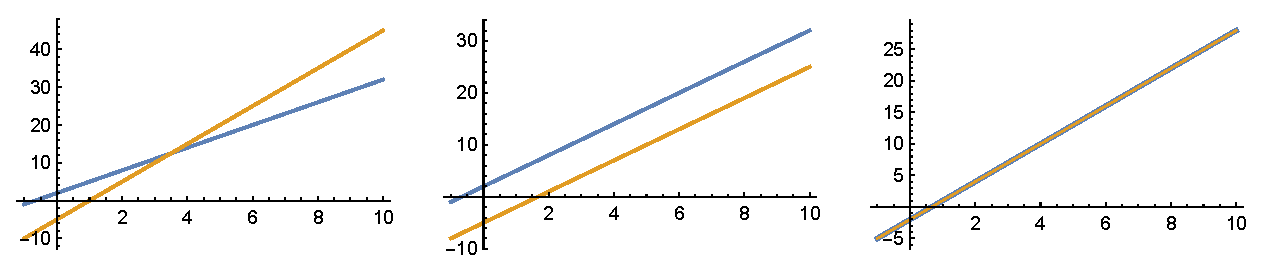
\includegraphics[scale=.8]{lines.eps}
\caption{A toy example of this algebra-geometry diction is that one can analyze a system of two linear equations, $ax+by=0, cx+dy=0$, by considering the graphs of the corresponding lines. In particular, by studying the corresponding lines one can see that a system of two linear equations $ax+by=0, cx+dy=0$ has exactly one, zero, or infinitely many solutions depending on whether the corresponding lines intersect, are parallel, or are the same line. }
\end{figure}
\end{center}
My research focuses on furthering our understanding of how algebraic relations between polynomials affects the geometry of their solution sets. Given a collection of polynomials $f_1,f_2,\ldots,f_{t}$, a \textit{syzygy} is another collection of polynomials $g_1,g_2,\ldots,g_{t}$ such that
$f_1g_1+f_2g_2+\cdots+f_{t}g_{t}=0$. Informally, a syzygy captures an algebraic relationship amoungst the polynomials $f_1,f_2,\ldots,f_t$. In my research, I have sought to understand the syzygies of a number of interesting varieties. 
 
The study of syzygies is formalized via commutative algebra in the following way. Given a graded module $M$ over a graded ring $R$, a helpful tool for understanding the structure of $M$ is its minimal graded free resolution. In essence, a minimal graded free resolution is a way of approximating $M$ by a sequence of free $R$-modules. More formally, a \textit{graded free resolution} of a module $M$ is an exact sequence 
\[
\cdots \xrightarrow{} F_{k} \xrightarrow{d_{k}} F_{k-1} \xrightarrow{d_{k-1}} \cdots \xrightarrow{d_{1}} F_{0}\xrightarrow{\epsilon}M\xrightarrow{} 0
\]
where each $F_{i}$ is a graded free $R$-module, and hence can be written as $\bigoplus_{j}R(-j)^{\beta_{i,j}}$. The module $R(-j)$ is the ring $R$ with a twisted grading, so that $R(-j)_{d}$ is equal to $R_{d-j}$ where $R_{d-j}$ is the graded piece of degree $d-j$. The $\beta_{i,j}$'s are the \textit{Betti numbers} of $M$, and they count the number of $i$-syzygies of $M$ of degree $j$. We will use syzygy and Betti number interchangeably throughout. 

Given a projective variety $X$ embedded in $\P^r$, we associate to $X$ the ring $S_X=S/I_X$, where $S=\C[x_0,\ldots,x_r]$ and $I_X$ is the ideal of homogenous polynomials vanishing on $X$. As $S_X$ is naturally a graded $S$-module we may consider its minimal graded free resolution, which is often closely related to both the extrinsic and intrinsic geometry of $X$.  An example of this phenomenon
 is Green's Conjecture, which relates the Clifford index of a curve with the vanishing of certain $\beta_{i,j}$ for its canonical embedding \cite{voisin02, voisin05, aproduFarkas19}. See also \cite{eisenbud05}*{Conjecture 9.6} and \cite{schreyer86, bayerEisenbud91,farkasPopa05, farkas06,aproduFarkas11,farkasKemeny16,farkasKemeny17}.

%\begin{theorem}[\cite{voisin02}, \cite{voisin05}]
%Let $C$ be a generic smooth projective curve of genus $g$ over a characteristic zero field embedded in $\P^{g-1}$ by the complete canonical series. Then the length of the first linear strand of the minimal free resolution of $I_X$ is $g-3-\text{Cliff}(C)$.
%\end{theorem}

\subsection{Asymptotic Syzygies}

Much of my work has focused on studying the asymptotic properties of syzygies of projective varieties. Broadly speaking, asymptotic syzygies is the study of the graded Betti numbers (i.e. the syzygies) of a projective variety as the positivity of the embedding grows. In many ways, this perspective dates back to classical work on the defining equations of curves of high degree and projective normality \cite{mumford66, mumford70}. However, the modern viewpoint arose from the pioneering work of Green \cite{green84-I, green84-II} and later Ein and Lazarsfeld \cite{einLazarsfeld12}. 

To give a flavor of the results of asymptotic syzygies we will focus on the question: In what degrees do non-zero syzygies occur? Going forward we will let $X\subset \P^{r_{d}}$ be a smooth projective variety embedded by a very ample line bundle $L_{d}$. Following \cite{ermanYang18} we set, 
\begin{align*}
\rho_q\left(X,L_{d}\right)\;\;\coloneqq&\ \;\; \frac{\#\left\{p\in\N |\; \big| \; \beta_{p,p+q}\left(X,L_{d}\right)\neq0\right\}}{r_{d}},
\end{align*}
which is the percentage of degrees in which non-zero syzygies appear \cite{eisenbud05}*{Theorem~1.1}. The asymptotic perspective asks how $\rho_{q}(X;L_{d})$ behaves along the sequence of line bundles $(L_{d})_{d\in \N}$. 
%\begin{align*}
%\rho_q\left(X;L_{d}\right)\;\;\coloneqq&\ \;\; \frac{\#\left\{p\in\N |\; \big| \; \beta_{p,p+q}\left(X,L_{d}\right)\neq0\right\}}{r_{d}}.
%\end{align*}
%which by the Hilbert Syzygy Theorem is the percentage of degrees in which non-zero syzygies appear \cite{eisenbud05}*{Theorem~1.1}. For any particular, $X$, $L_{d}$, and $q$ computing $\rho_{q}(X;L_{d})$ is often quite difficult. The asymptotic perspective thus, asks instead, to consider a sequence of line bundles $(L_{d})_{d\in \N}$ and ask how $\rho_{q}(X;L_{d})$ behaves along the sequence of $(L_{d})_{d\in \N}$. 

With this notation in hand, we may phrase Green's work on the vanishing of syzygies for curves of high degree as computing the asymptotic percentage of non-zero quadratic syzygies. 

\begin{theorem}\cite{green84-I}
Let $X\subset \P^r$ be a smooth projective curve. If $(L_{d})_{d\in\N}$ is a sequence of very ample line bundles on $X$ such that $\deg L_{d} = d$ then 
\[
\lim_{d\to \infty} \rho_{2}\left(X;L_{d}\right) = 0.
\]
\end{theorem}

Put differently, asymptotically the syzygies of curves are as simple as possible, occurring in the lowest possible degree. This inspired substantial work, with the intuition being that syzygies become simpler as the positivity of the embedding increases \cite{ottavianiPaoletti01, einLazarsfeld93, lazarsfeldPareschiPopa11, pareschi00, pareschiPopa03, pareschiPopa04}.  

In a groundbreaking paper, Ein and Lazarsfeld showed that for higher dimensional varieties this intuition is often misleading. Contrary to the case of curves, they show that for higher dimensional varieties, asymptotically syzygies appear in every possible degree. 
  
\begin{theorem}\cite{einLazarsfeld12}*{Theorem~C}
Let $X\subset \P^r$ be a smooth projective variety, $\dim X \geq2$, and fix an index $1\leq q \leq \dim X$. If $(L_{d})_{d\in\N}$ is a sequence of very ample line bundles such that $L_{d+1}-L_{d}$ is constant and ample then
\[
\lim_{d\to\infty} \rho_{q}\left(X; L_d\right) = 1.
\]
\end{theorem}

My work has focused on the behavior of asymptotic syzygies when the condition that $L_{d+1}-L_{d}$ is constant and ample is weakened to assuming $L_{d+1}-L_{d}$ is semi-ample. Recall a line bundle $L$ is \textit{semi-ample} if $|kL|$ is base point free for $k\gg0$. The prototypical example of a semi-ample line bundle is $\O(1,0)$ on $\P^{n}\times \P^{m}$. My exploration of asymptotic syzygies in the setting of semi-ample growth thus began by proving the following nonvanishing result for $\P^{n}\times\P^{m}$ embedded by $\O(d_{1},d_{2})$. 

\begin{theorem}\cite{bruce19-semiample}*{Corollary~B}\label{thm:bruce-semiample}
Let $X=\P^{n}\times\P^{m}$ and fix an index $1\leq q \leq n+m$. There exist constants $C_{i,j}$ and $D_{i,j}$ such that
\[
\rho_{q}\left(X; \O\left(d_1,d_2\right)\right)\geq1-\sum_{\substack{i+j=q \\  i \leq n, \; j \leq m}}\left(
\frac{C_{i,j}}{d_1^id_2^j}+\frac{D_{i,j}}{d_1^{n-i}d_2^{m-j}}\right)-O\left(\begin{matrix}\text{lower ord.}\\ \text{terms}\end{matrix}\right).
\]
\end{theorem}

Notice if both $d_{1}\to \infty$ and $d_{2}\to\infty$ then $\rho_{q}\left(\P^{n}\times\P^{m}; \O(d_1,d_2)\right)\to1$, recovering the results of Ein and Lazarsfeld for $\P^n\times\P^m$. However, if $d_{1}$ is fixed and $d_{2}\to \infty$ (i.e. semi-ample growth) my results bound the asymptotic percentage of non-zero syzygies away from zero. This together with work of Lemmens \cite{lemmens18} has led me to conjecture that, unlike in previously studied cases, in the semi-ample setting $\rho_{q}\left(\P^{n}\times\P^{m}; \O(d_1,d_2)\right)$ does not approach 1. Proving this would require a vanishing result for asymptotic syzygies, which is open even in the ample case  \cite[Conjectures~7.1,~7.5]{einLazarsfeld12}.


% In particular, the asymptotic behavior is dependent, in a nuanced way, on the relationship between $d_{1}$ and $d_{2}$. 

%For example, considering $\P^{1}\times\P^{5}$ and $q=2$ then Theorem~\ref{thm:bruce-semiample} shows that 
%\[
%\rho_{2}\left(\P^{1}\times\P^{5}; \O(d_1,d_2)\right)\geq1-\frac{20}{d_2^2}-\frac{60}{d_1d_2^3}-\frac{5}{d_1d_2}-\frac{120}{d_2^4}-O\left(\begin{matrix}\text{lower ord.}\\ \text{terms}\end{matrix}\right)\,.
%\]
%Moreover, if $d_2$ is fixed and $d_1\to\infty$, then the limit of $\rho_{2}\left(\P^{1}\times\P^{5}; \O(d_1,d_2)\right)$ is greater than or equal to $1-\frac{20}{d^2_2}-\frac{120}{d_2^4}$.

%Results of Lemmens in the case of $\P^1\times\P^1$ together with my work has led me to conjecture that unlike in previously study cases (i.e. curves and ample growth) in the case of semi-ample growth $\rho_{q}\left(\P^{n}\times\P^{m}; \O(d_1,d_2)\right)$ does not approach 1 as $d_{1}\to \infty$. Proving this would require a vanishing result for asymptotic syzygies, which is open even in the ample case. See \cite[Conjecture~7.1, Conjecture~7.5]{einLazarsfeld12}.

The proof of Theorem~\ref{thm:bruce-semiample} is based upon generalizing the monomial methods of Ein, Erman, and Lazarsfeld. Such a generalization is complicated by the difference between the Cox ring and homogenous coordinate ring of $\P^{n}\times\P^{m}$. A central theme in this work is to exploit the fact that a key regular sequence I use has a number of non-trivial symmetries. 
%These symmetries, when combined with a series of spectral sequence arguments, allow me to prove Theorem~\ref{thm:bruce-semiample}.

This work suggests that the theory of asymptotic syzygies in the setting of semi-ample growth is rich and substantially different from the other previously studied cases. Going forward I plan to use this work as a jumping-off point for the following question.  

\begin{question}\label{quest:semi-ample}
Let $X\subset \P^{r_d}$ be a smooth projective variety and fix an index $1\leq q \leq \dim X$. Let $(L_{d})_{d\in\N}$ be a sequence of very ample line bundles such that $L_{d+1}-L_{d}$ is constant and semi-ample, can one compute $\lim_{d\to\infty} \rho_{q}\left(X;L_{d}\right)$?
\end{question}

A natural next case in which to consider Question~\ref{quest:semi-ample} is that of Hirzebruch surfaces. I addressed a different, but related question for a narrow class of Hirzebruch surfaces in \cite{bruce19-hirzebruch}.

\subsection{Syzygies via Highly Distributed Computing}

It is quite difficult to compute examples of syzygies. For example, until recently the syzygies of the projective plane embedded by the $d$-uple Veronese embedding were only known for $d\leq 5$. My co-authors and I exploited recent advances in numerical linear algebra and high-throughput high-performance computing to generate a number of new examples of Veronese syzygies. This data provided support for several existing conjectures, as well as led us to make a number of new conjectures \cite{bruceErmanGoldsteinYang18}. 
The resulting data has been made publicly available via SyzygyData.com as well as, a package for Macaualy2 \cite{bruceErman19, M2}.

%This is because while the problem of computing syzygies can be reduced to computing ranks of matrices, the number of matrices and their sizes quickly become extremely large. As an example, to compute the syzygies of $\P^2$ embedded by the $6$-uple Veronese embedding there are well over 6,000 relevant matrices with the around 2,000 of them being on the order of $4,000,000 \times 12,000,000$. 


Recently I have begun using similar computational techniques to compute the syzygies for Hirzebruch surfaces. Thus far, we have computed the syzygies in  $\sim100$ new examples. It is our hope that these examples will lead to new conjectures regarding the syzygies of Hirzebruch surfaces. In particular, we believe our data will be useful in addressing Question~\ref{quest:semi-ample}. 

\begin{bibdiv}
\begin{biblist}[\normalsize]
      \bib{almousaBruce19}{article}{
   author={Almousa, Ayah},
   author={Bruce, Juliette},
   author={Loper, Michael C.},
   author={Sayrafi, Mahrud},
   title={The virtual resolutions package for Macaulay2},
   date={2019},
   note={Pre-print: \href{https://arxiv.org/abs/1905.07022}{arxiv:1905.07022}}
   }
   
\bib{aproduFarkas19}{article}{
   author={Aprodu, Marian},
   author={Farkas, Gavrill},
   author={Papadima, {\c{S}}tefan},
   author={Raicu, Claudiu},
   author={Weyman, Jerzy},
   title={Koszul modules and Green's conjecture},
   journal={Inventiones mathematicae},
   year={2019},
   month={Jun}
   day={15}
%   issn={1432-1297},
%   doi={10.1007/s00222-019-00894-1},
}

\bib{aproduFarkas11}{article}{
   author={Aprodu, Marian},
   author={Farkas, Gavril},
   title={Green's conjecture for curves on arbitrary $K3$ surfaces},
   journal={Compos. Math.},
   volume={147},
   date={2011},
   number={3},
   pages={839--851},
   issn={0010-437X},
   review={\MR{2801402}},
   doi={10.1112/S0010437X10005099},
}


\bib{bayerEisenbud91}{article}{
   author={Bayer, Dave},
   author={Eisenbud, David},
   title={Graph curves},
   note={With an appendix by Sung Won Park},
   journal={Adv. Math.},
   volume={86},
   date={1991},
   number={1},
   pages={1--40},
%   issn={0001-8708},
%   review={\MR{1097026}},
%   doi={10.1016/0001-8708(91)90034-5},
}


\bib{bruceErman-sop}{article}{
   author={Bruce, Juliette},
   author={Erman, Daniel},
   title={A probabilistic approach to systems of parameters and Noether normalization },
   journal={Algebra Number Theory},
   note={to appear}
}

\bib{bruceLi19}{article}{
   author={Bruce, Juliette},
   author={Li, Wanlin},
   title={Effective bounds on the dimensions of jacobians covering abelian varieties },
   journal={Proc. Amer. Math. Soc.},
   note={to appear}
}

\bib{bruceErmanGoldsteinYang18}{article}{
	author = {Bruce, Juliette},
	author = {Erman, Daniel},
	author = {Goldstein. Steve}, 
	author = {Yang, Jay},
	title = {Conjectures and computations about Veronese syzygies},
	journal = {Experimental Mathematics},
	volume = {0},
	number = {0},
	pages = {1-16},
	year  = {2018}
	}

   \bib{bruceErman19}{article}{
   author={Bruce, Juliette},
   author = {Erman, Daniel},
   author = {Goldstein. Steve}, 
   author = {Yang, Jay},
   title={The SchurVeronese package in Macaulay2},
   date={2019},
   note={Pre-print: \href{https://arxiv.org/abs/1905.12661}{arxiv:1905.12661}}
   }

\bib{bruce19-semiample}{article}{
   author={Bruce, Juliette},
   title={Asymptotic syzygies in the setting of semi-ample growth},
   date={2019},
   note={Pre-print: \href{https://arxiv.org/abs/1904.04944}{arxiv:1904.04944}}
   }

\bib{bruce19-hirzebruch}{article}{
   author={Bruce, Juliette},
   title={The quantitative behavior of asymptotic syzygies for Hirzebruch surfaces},
   date={2019},
   note={Pre-print: \href{https://arxiv.org/abs/1906.07333}{arxiv:1906.07333}}
   }
   
\bib{caldararu10}{article}{
   author={C\u{a}ld\u{a}raru, Andrei},
   author={Distler, Jacques},
   author={Hellerman, Simeon},
   author={Pantev, Tony},
   author={Sharpe, Eric},
   title={Non-birational twisted derived equivalences in abelian GLSMs},
   journal={Comm. Math. Phys.},
   volume={294},
   date={2010},
   number={3},
   pages={605--645},
   issn={0010-3616},
   review={\MR{2585982}},
   doi={10.1007/s00220-009-0974-2},
}


%\bib{charlesPoonen16}{article}{
%   author={Charles, Fran\c{c}ois},
%   author={Poonen, Bjorn},
%   title={Bertini irreducibility theorems over finite fields},
%   journal={J. Amer. Math. Soc.},
%   volume={29},
%   date={2016},
%   number={1},
%   pages={81--94},
%   issn={0894-0347},
%   review={\MR{3402695}},
%   doi={10.1090/S0894-0347-2014-00820-1},
%}
\bib{chenEurYangZhang19}{article}{
    author={Chen, Justin},
    author={Eur, Christopher},
    author={Yang, Greg},
    author={Zhang, Mengyuan},
    title={Free resolutions of function classes via order complexes},
    year={2019},
    eprint={1909.02159},
    archivePrefix={arXiv},
}

\bib{craciun15}{article}{
   author={Craciun, Gheorghe},
   title={Toric Differential Inclusions and a Proof of the Global Attractor Conjecture},
   year={2015},
   eprint={1501.02860},
    archivePrefix={arXiv},
}

\bib{einLazarsfeld93}{article}{
   author={Ein, Lawrence},
   author={Lazarsfeld, Robert},
   title={Syzygies and Koszul cohomology of smooth projective varieties of
   arbitrary dimension},
   journal={Invent. Math.},
   volume={111},
   date={1993},
   number={1},
   pages={51--67},
%   issn={0020-9910},
%   review={\MR{1193597}},
%   doi={10.1007/BF01231279},
}
	
				
%\bib{einErmanLazarsfeld15}{article}{
%   author={Ein, Lawrence},
%   author={Erman, Daniel},
%   author={Lazarsfeld, Robert},
%   title={Asymptotics of random Betti tables},
%   journal={J. Reine Angew. Math.},
%   volume={702},
%   date={2015},
%   pages={55--75},
%   issn={0075-4102},
%   review={\MR{3341466}},
%   doi={10.1515/crelle-2013-0032},
%}

\bib{einLazarsfeld12}{article}{
   author={Ein, Lawrence},
   author={Lazarsfeld, Robert},
   title={Asymptotic syzygies of algebraic varieties},
   journal={Invent. Math.},
   volume={190},
   date={2012},
   number={3},
   pages={603--646},
%   issn={0020-9910},
%   review={\MR{2995182}},
%   doi={10.1007/s00222-012-0384-5},
}

\bib{eisenbud05}{book}{
   author={Eisenbud, David},
   title={The geometry of syzygies},
   series={Graduate Texts in Mathematics},
   volume={229},
   note={A second course in commutative algebra and algebraic geometry},
   publisher={Springer-Verlag, New York},
   date={2005},
   pages={xvi+243},
%   isbn={0-387-22215-4},
%   review={\MR{2103875}},
}
%
%
%\bib{eisenbudSchreyer09}{article}{
%   author={Eisenbud, David},
%   author={Schreyer, Frank-Olaf},
%   title={Betti numbers of graded modules and cohomology of vector bundles},
%   journal={J. Amer. Math. Soc.},
%   volume={22},
%   date={2009},
%   number={3},
%   pages={859--888},
%%   issn={0894-0347},
%%   review={\MR{2505303}},
%%   doi={10.1090/S0894-0347-08-00620-6},
%}

\bib{ermanYang18}{article}{
   author={Erman, Daniel},
   author={Yang, Jay},
   title={Random flag complexes and asymptotic syzygies},
   journal={Algebra Number Theory},
   volume={12},
   date={2018},
   number={9},
   pages={2151--2166},
%   issn={1937-0652},
%   review={\MR{3894431}},
%   doi={10.2140/ant.2018.12.2151},
}

\bib{farkasPopa05}{article}{
   author={Farkas, Gavril},
   author={Popa, Mihnea},
   title={Effective divisors on $\overline{\mathcal{M}}_g$, curves on $K3$
   surfaces, and the slope conjecture},
   journal={J. Algebraic Geom.},
   volume={14},
   date={2005},
   number={2},
   pages={241--267},
%   issn={1056-3911},
%   review={\MR{2123229}},
%   doi={10.1090/S1056-3911-04-00392-3},
}

\bib{farkas06}{article}{
   author={Farkas, Gavril},
   title={Syzygies of curves and the effective cone of $\overline{
  \mathcal{M}}_g$},
   journal={Duke Math. J.},
   volume={135},
   date={2006},
   number={1},
   pages={53--98},
%   issn={0012-7094},
%   review={\MR{2259923}},
%   doi={10.1215/S0012-7094-06-13512-3},
}

\bib{farkasKemeny16}{article}{
   author={Farkas, Gavril},
   author={Kemeny, Michael},
   title={The generic Green-Lazarsfeld secant conjecture},
   journal={Invent. Math.},
   volume={203},
   date={2016},
   number={1},
   pages={265--301},
%   issn={0020-9910},
%   review={\MR{3437872}},
%   doi={10.1007/s00222-015-0595-7},
}

\bib{farkasKemeny17}{article}{
   author={Farkas, Gavril},
   author={Kemeny, Michael},
   title={The Prym-Green conjecture for torsion line bundles of high order},
   journal={Duke Math. J.},
   volume={166},
   date={2017},
   number={6},
   pages={1103--1124},
%   issn={0012-7094},
%   review={\MR{3635900}},
%   doi={10.1215/00127094-3792814},
}

\bib{green84-I}{article}{
   author={Green, Mark L.},
   title={Koszul cohomology and the geometry of projective varieties},
   journal={J. Differential Geom.},
   volume={19},
   date={1984},
   number={1},
   pages={125--171},
%   issn={0022-040X},
%   review={\MR{739785}},
}

\bib{green84-II}{article}{
   author={Green, Mark L.},
   title={Koszul cohomology and the geometry of projective varieties. II},
   journal={J. Differential Geom.},
   volume={20},
   date={1984},
   number={1},
   pages={279--289},
%   issn={0022-040X},
%   review={\MR{772134}},
}
	
\bib{lazarsfeldPareschiPopa11}{article}{
   author={Lazarsfeld, Robert},
   author={Pareschi, Giuseppe},
   author={Popa, Mihnea},
   title={Local positivity, multiplier ideals, and syzygies of abelian
   varieties},
   journal={Algebra Number Theory},
   volume={5},
   date={2011},
   number={2},
   pages={185--196},
%   issn={1937-0652},
%   review={\MR{2833789}},
%   doi={10.2140/ant.2011.5.185},
}

\bib{lemmens18}{article}{
   author={Lemmens, Alexander},
   title={On the $n$-th row of the graded Betti table of an $n$-dimensional
   toric variety},
   journal={J. Algebraic Combin.},
   volume={47},
   date={2018},
   number={4},
   pages={561--584},
%   issn={0925-9899},
%   review={\MR{3813640}},
%   doi={10.1007/s10801-017-0786-y},
}


\bib{M2}{misc}{
    label={M2},
    author={Grayson, Daniel~R.},
    author={Stillman, Michael~E.},
    title = {Macaulay 2, a software system for research
	    in algebraic geometry},
    note = {Available at \url{http://www.math.uiuc.edu/Macaulay2/}},
}

\bib{mumford70}{article}{
   author={Mumford, David},
   title={Varieties defined by quadratic equations},
   conference={
      title={Questions on Algebraic Varieties},
      address={C.I.M.E., III Ciclo, Varenna},
      date={1969},
   },
   book={
      publisher={Edizioni Cremonese, Rome},
   },
   date={1970},
   pages={29--100},
%   review={\MR{0282975}},
}
	
\bib{mumford66}{article}{
   author={Mumford, D.},
   title={On the equations defining abelian varieties. I},
   journal={Invent. Math.},
   volume={1},
   date={1966},
   pages={287--354},
%   issn={0020-9910},
%   review={\MR{204427}},
%   doi={10.1007/BF01389737},
}
	
%	\bib{oeding17}{article}{
%   author={Oeding, Luke},
%   author={Raicu, Claudiu},
%   author={Sam, Steven V},
%   title={On the (non-)vanishing of syzygies of Segre embeddings},
%   journal={Algebraic Geometry},
%   volume={6},
%   number={5},
%   date={2019},
%   pages={571--591},
%}

\bib{ottavianiPaoletti01}{article}{
   author={Ottaviani, Giorgio},
   author={Paoletti, Raffaella},
   title={Syzygies of Veronese embeddings},
   journal={Compositio Math.},
   volume={125},
   date={2001},
   number={1},
   pages={31--37},
%   issn={0010-437X},
%   review={\MR{1818055}},
%   doi={10.1023/A:1002662809474},
}
	
\bib{pareschi00}{article}{
   author={Pareschi, Giuseppe},
   title={Syzygies of abelian varieties},
   journal={J. Amer. Math. Soc.},
   volume={13},
   date={2000},
   number={3},
   pages={651--664},
%   issn={0894-0347},
%   review={\MR{1758758}},
%   doi={10.1090/S0894-0347-00-00335-0},
}

\bib{pachterSturmfels05}{collection}{
   title={Algebraic statistics for computational biology},
   editor={Pachter, Lior},
   editor={Sturmfels, Bernd},
   publisher={Cambridge University Press, New York},
   date={2005},
   pages={xii+420},
   isbn={978-0-521-85700-0},
   isbn={0-521-85700-7},
   review={\MR{2205865}},
   doi={10.1017/CBO9780511610684},
}
	
\bib{pareschiPopa03}{article}{
   author={Pareschi, Giuseppe},
   author={Popa, Mihnea},
   title={Regularity on abelian varieties. I},
   journal={J. Amer. Math. Soc.},
   volume={16},
   date={2003},
   number={2},
   pages={285--302},
%   issn={0894-0347},
%   review={\MR{1949161}},
%   doi={10.1090/S0894-0347-02-00414-9},
}


\bib{pareschiPopa04}{article}{
   author={Pareschi, Giuseppe},
   author={Popa, Mihnea},
   title={Regularity on abelian varieties. II. Basic results on linear
   series and defining equations},
   journal={J. Algebraic Geom.},
   volume={13},
   date={2004},
   number={1},
   pages={167--193},
%   issn={1056-3911},
%   review={\MR{2008719}},
%   doi={10.1090/S1056-3911-03-00345-X},
}

\bib{schreyer86}{article}{
   author={Schreyer, Frank-Olaf},
   title={Syzygies of canonical curves and special linear series},
   journal={Math. Ann.},
   volume={275},
   date={1986},
   number={1},
   pages={105--137},
%   issn={0025-5831},
%   review={\MR{849058}},
%   doi={10.1007/BF01458587},
}	
	
\bib{voisin02}{article}{
   author={Voisin, Claire},
   title={Green's generic syzygy conjecture for curves of even genus lying
   on a $K3$ surface},
   journal={J. Eur. Math. Soc. (JEMS)},
   volume={4},
   date={2002},
   number={4},
   pages={363--404},
%   issn={1435-9855},
%   review={\MR{1941089}},
%   doi={10.1007/s100970200042},
}

\bib{voisin05}{article}{
   author={Voisin, Claire},
   title={Green's canonical syzygy conjecture for generic curves of odd
   genus},
   journal={Compos. Math.},
   volume={141},
   date={2005},
   number={5},
   pages={1163--1190},
%   issn={0010-437X},
%   review={\MR{2157134}},
%   doi={10.1112/S0010437X05001387},
}
	
\end{biblist}
\end{bibdiv}

%%%%%%%%%%%%%%%%%%%%%%%%%%%%%%%%%%%%%%%%%%%%%%%%%%%%%%%%%%%%%%%%%%%%%%%%%%%%%%%%%%%%%%%%%%%%%%%%%%%%%%%%%%


\end{document}